Für die Bestimmung des Templates des korrelierten Untergrunds wird das Template des Signals von einer Verteilung der invarianter Masse abgezogen, die im gleichen $p_\text{T}$-Intervall liegt, wie das Template des Signals.
Die Verteilung der invarianter Masse kommt dabei aus der Monte Carlo Simulation, auf die das Analyseverfahren bis einschließlich der Abschätzung der unkorrelierten Untergrunds angewandt wurde.
\begin{figure}[tp]
\centering
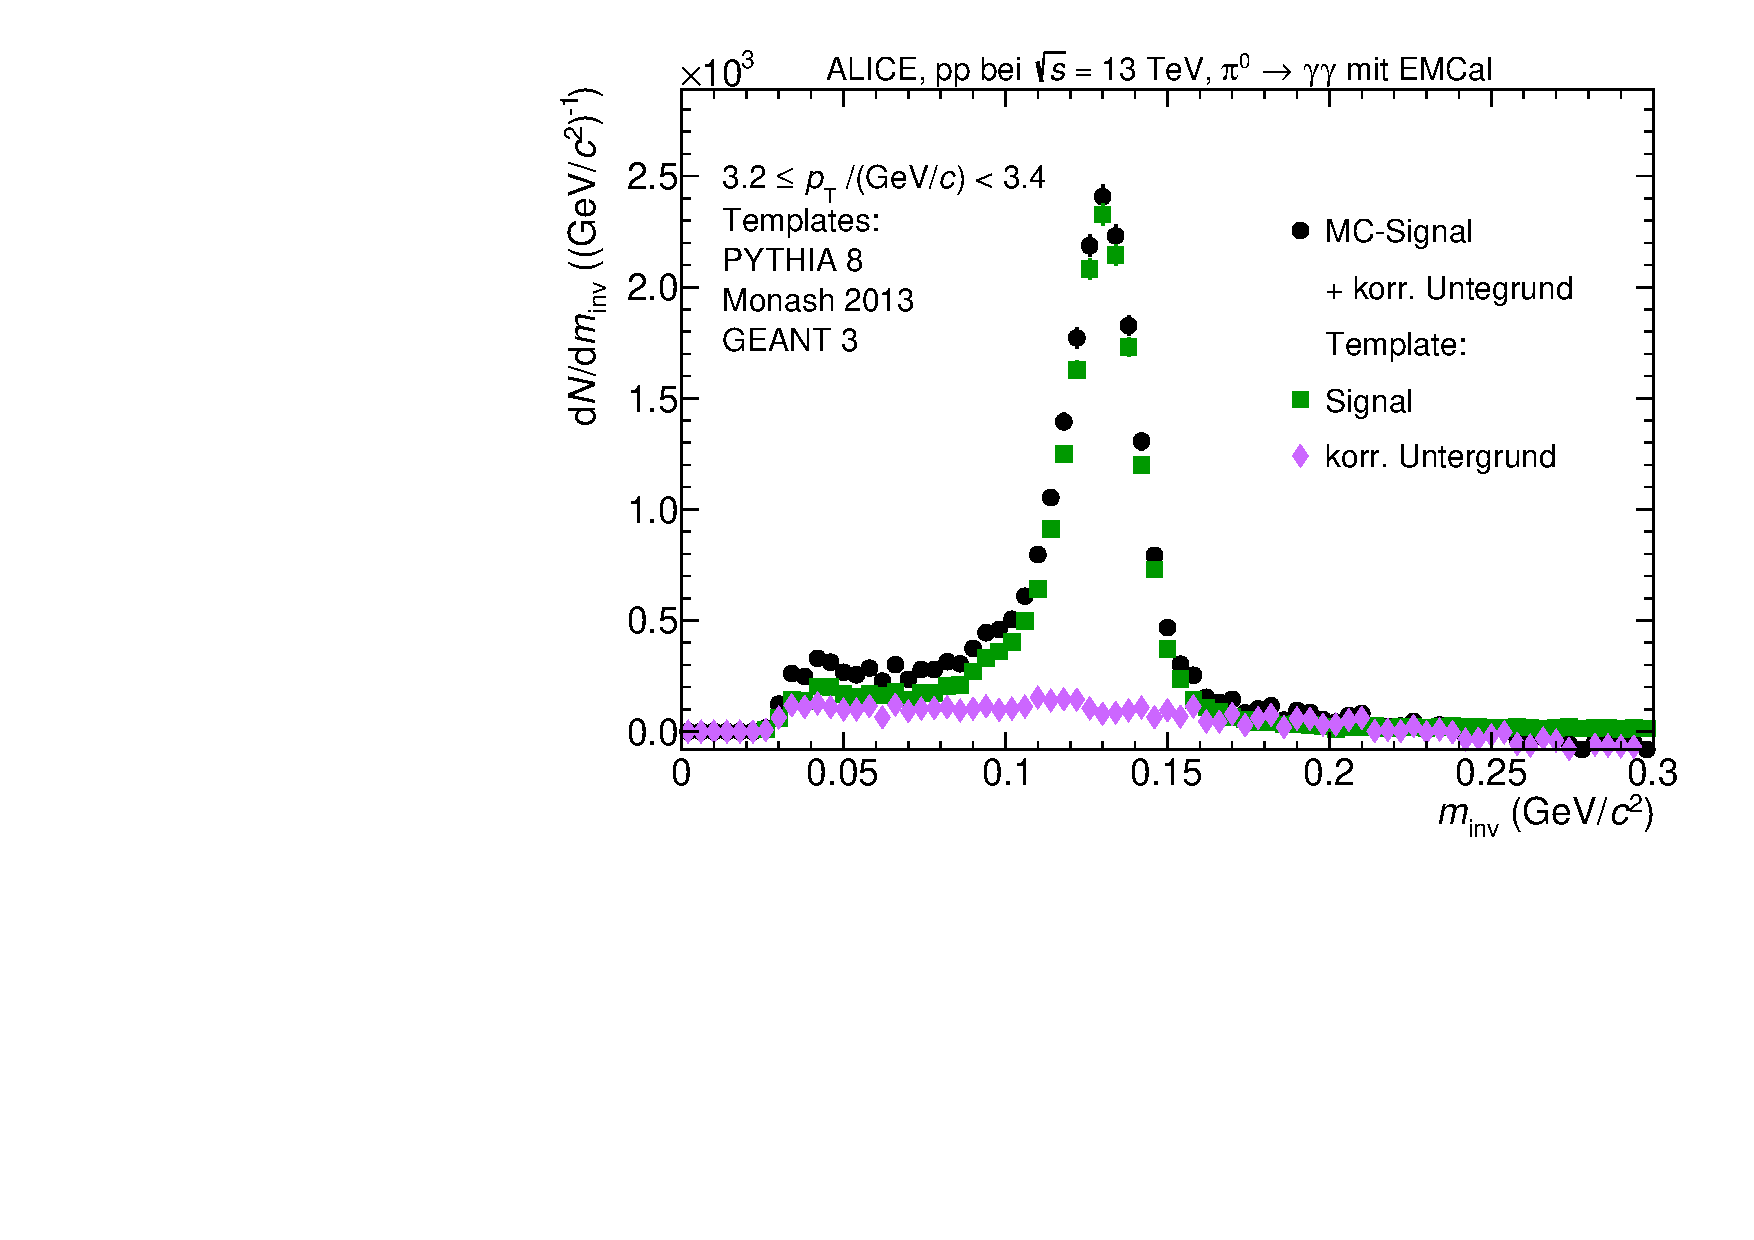
\includegraphics[width=.75\linewidth]{EntstehungUntergrund10_Data_2016.pdf}
\caption{Template des korrelierten Untergrunds in pink entstanden durch den Abzug des Templates des Signals (grün) von der Verteilung der invarianten Masse aus einer Monte Carlo Simulation (schwarz).}
\label{fig:BkgTemp}
\end{figure}
\newline
Abbildung \ref{fig:BkgTemp} zeigt in pink das Template des korrelierten Untergrunds für das $p_\text{T}$-Intervall $(3\,2 - 3\,4) (\text{GeV/}c)$.
Zur Verdeutlichung sind ebenfalls das oben beschriebene Signal in schwarz und das Template des Signals in grün eingezeichnet.
\newline
Für großes $p_\text{T}$ wird die Unsicherheit im Template des korrelierten Untergrunds relativ groß im Vergleich mit der Anzahl an Einträgen in der Verteilung der invarianten Masse.
Innerhalb der Unsicherheiten liegen die Werte der Templates des korrelierten Untergrunds dann bei Null, was eine Anpassung an die Daten, unter Berücksichtigung der statistischen Unsicherheiten, erschwert.
%^geht das so^?
Um die Unsicherheit zu verkleinern wird in dieser Arbeit der korrelierte Untergrund aus mehreren $p_\text{T}$-Intervallen zusammengefasst, in ein kombiniertes Template des korrelierten Untergrunds.
Dabei wird angenommen, dass sich nicht die Form, sondern nur die Anzahl der Einträge in den $p_\text{T}$-Intervallen unterscheidet.  
Für die Zusammenfassung der Templates des korrelierten Untergrunds werden die Templates des korrelierten Untergrunds aus den $p_\text{T}$-Intervallen von $p_\text{T} \geq 1\,8\text{ GeV}/c$ bis $p_\text{T} \leq 3\,2\text{ GeV}/c$ benutzt, da sie die geringsten statistischen Unsicherheiten besitzen.
Diese werden zunächst aufsummiert und auf die Anzahl der verwendeten $p_\text{T}$-Intervalle normiert.
\begin{figure}[tp]
\centering
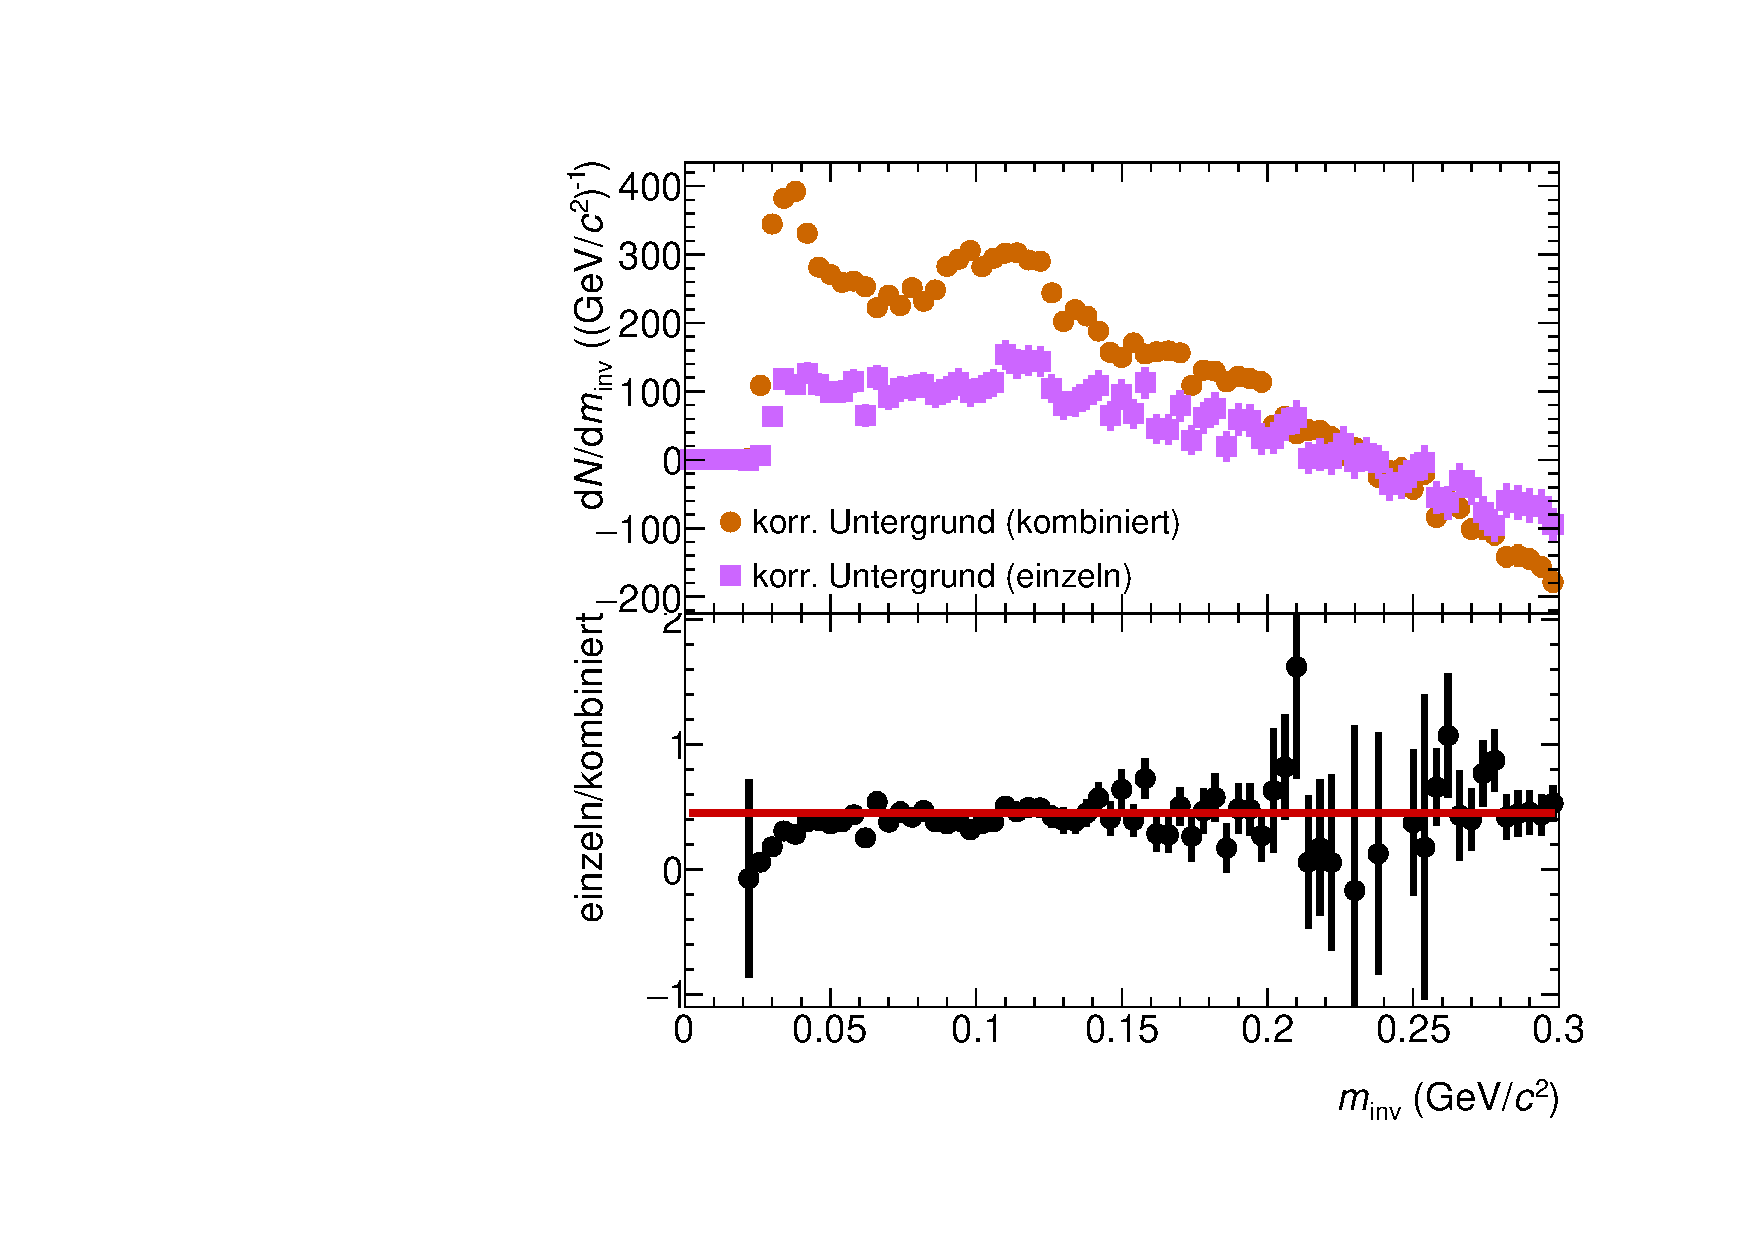
\includegraphics[width=.7\linewidth]{BackgroundWithRatio10_Data_2016.pdf}
\caption{\textbf{Oben:} Template des korrelierten Untergrunds aus einem einzelnen $p_\text{T}$-Intervall in pink und aus mehreren $p_\text{T}$-Intervallen kombiniert in orange.
\textbf{Unten:} Verhältnis der beiden Verteilungen in schwarz, sowie Parametrisierung einer Konstante an das Verhältnis in rot.}
\label{fig:BkgTempRatio}
\end{figure}
\newline
Abbildung \ref{fig:BkgTempRatio} zeigt in orange ein kombiniertes Template des korrelierten Untergrunds und in pink das Template des korrelierten Untergrunds für das $p_\text{T}$-Intervall $(3\,2 - 3\,4) (\text{GeV/}c)$.
Um zu zeigen, dass die Annahme ihre Richtigkeit hat wird in Abbildung \ref{fig:BkgTempRatio} das Verhältnis aus einzelnem Template des korrelierten Untergrunds zu den Kombinierten dargestellt.
Die rote Linie im unteren Teil der Abbildung basiert auf einer konstanten Parametrisierung des Verhältnisses.
Die getroffene Annahme wird bestätigt, da die konstante Parametrisierung und das Verhältnis gut miteinander übereinstimmen.
Die großen Unsicherheiten im Verhältnis um $m_\text{inv} = 0,225\text{ GeV}/c^{2}$ entsteht, da beide Templates an dieser Stelle eine Anzahl an Einträgen im Bereich nah um die Null besitzen.
Teilt man zwei kleine Zahlen durch einander, so ändert sich der Quotientenwert stark, wenn man nur eine der beiden kleinen Zahlen leicht ändert.
Dadurch wird auch die Unsicherheit auf den Quotientenwert deutlich größer.
\newline
Zuvor wurde bereits angesprochen, dass die Anforderung an den Öffnungswinkel abhängig von $p_\text{T}$ ist.
Um das kombinierte Template des korrelieren Untergrunds daran anzupassen wurde eine vereinfachte Monte Carlo Simulation durchgeführt.
Die Simulation beinhaltete zwei Teile, in beiden Teilen wurden Teilchen mit zufälliger Energie simuliert, die in zwei Photonen zerfallen.
Die Photonen müssen dann auf einen Fläche auftreten die der Fläche des EMCals entspricht, um als detektiert zu gelten.
Dabei werden in beiden Teilsimulationen so viele Teilchen produziert, dass die selbe Anzahl an Photonen auf die Fläche des EMCals trifft.
Anschließend werden die Photonen paarweise miteinander kombiniert, für jeden Teil der Simulation separat.
In einer der beiden Simulationsteile werden dabei die Anforderung an den Öffnungswinkel noch zusätzlich gestellt, wodurch bei der paarweisen Kombination der Photonen einige Paare ausgeschlossen werden.
Daraus entstehen zwei Verteilungen, die die Anzahl kombinierter Photonenpaare als Funktion von $m_\text{inv}$ und $p_\text{T}$ darstellen, einmal für den Fall, dass es keine Anforderung an den Öffnungswinkel gibt und einmal mit der Anforderung an den Öffnungswinkel.
Da beide Teilsimulationen die gleiche Anzahl an detektierten Photonen haben, kann aus dem Verhältnis der Verteilung mit Anforderung an den Öffnungswinkel zur Verteilung ohne Anforderung an den Öffnungswinkel, bestimmt werden, wie wahrscheinlich es ist einen Photonenkombination bei einem bestimmen $m_\text{inv}$ und $p_\text{T}$ zu messen.
Mit Hilfe dieser Wahrscheinlichkeitsverteilung werden die Templates des korrelierten Untergrunds, die das kombinierte Template des korrelierten Untergrunds bilden, an die unterschiedlichen $p_\text{T}$-Intervalle skaliert.
Dadurch konnten größere Abweichungen für kleinere invariante Massen vermieden werden.
\newline
In Abschnitt \ref{s4s2} wird für die Bestimmung der systematischen Unsicherheit die Wahl des Templates des korrelierten Untergrunds variiert.
\newline
Zum einen werden die Templates einzeln verwendet, also jeweils das Template des korrelierten Untergrunds aus dem jeweiligen $p_\text{T}$-Intervall, aus dem auch die Verteilung der invarianten Masse und das Template des Signals kommen.
Somit 
Wie bereits erwähnt wird die statistisch Unsicherheit, relativ gesehen zu den Werten der Templates, groß.
Das hat zur Folge, dass je stärker das Template des korrelierten Untergrunds skaliert wird, desto größer werden die statistischen Unsicherheiten.
Die statistischen Unsicherheiten sind jedoch immer groß genug, sodass die Werte des Template des korrelierten Untergrunds mit Null kompatibel sind.
Effektiv wird nur die statistische Unsicherheit erhöht, was $\chi^{2}$ verkleinert.
Dadurch wird die Anpassung über $\chi^{2}$-Minimierung verfälscht.
Die Berechnung von $\chi^{2}$ wird im nächsten Abschnitt genauer erläutert.
\newline
Zum anderen wird die Kombination variiert, sodass das Template des korrelierten Untergrunds nicht aus einem festen vergrößerten $p_\text{T}$-Intervall stammt.
Stattdessen wird das $p_\text{T}$-Intervall eines einzelnen Templates des korrelierten Untergrunds ausgeweitet, bis das Intervall mindestens $4\text{ GeV}/c$ umfasst.
Die Annahme, dass sich die Form der korrelierten Untergrunds nicht ändert, kann dabei aufgelockert werden, da nur benachbarte $p_\text{T}$-Intervall kombiniert werden.
Es wäre also akzeptabel, wenn sich die Form verändert, solange die Änderung kontinuierlich und langsam statt findet.
Die dadurch entstehende Korrelation in den statistischen Unsicherheiten der verschiedenen kombinierten Templates des korrelierten Untergrunds kann dabei nur grob abgeschätzt werden. 
\newline
Aus den genannten negativ Gründen, sowie der Bestätigung der Annahme, dass die Form des korrelierten Untergrund nicht von $p_\text{T}$ abhängt, werden beide Methoden für die Bestimmung der systematischen Unsicherheiten benutzt und nicht als Standard.
\newline
Im Folgenden Abschnitt werden die Templates des Signals und des korrelierten Untergrunds so parametrisiert, dass sie die Daten nach Abschätzung des unkorrelierten Untergrunds bestmöglich beschreiben.